\documentclass[10pt]{article}
\usepackage[letterpaper]{geometry}
\geometry{verbose,tmargin=1in,bmargin=1in,lmargin=1in,rmargin=1in}
\usepackage{setspace}
\usepackage{ragged2e}
\usepackage{color}
\usepackage{titlesec}
\usepackage{graphicx}
\usepackage{float}
\usepackage{mathtools}
\usepackage{amsmath}
\usepackage[font=small,labelfont=bf,labelsep=period]{caption}
\usepackage[english]{babel}
\usepackage{indentfirst}
\usepackage{array}
\usepackage{makecell}
\usepackage[usenames,dvipsnames]{xcolor}
\usepackage{multirow}
\usepackage{tabularx}
\usepackage{arydshln}
\usepackage{caption}
\usepackage{subcaption}
\usepackage{xfrac}
\usepackage{etoolbox}
\usepackage{cite}
\usepackage{url}
\usepackage{dcolumn}
\usepackage{hyperref}
\usepackage{courier}
\usepackage{url}
\usepackage{esvect}
\usepackage{commath}
\usepackage{verbatim} % for block comments
\usepackage{enumitem}
\usepackage{hyperref} % for clickable table of contents
\usepackage{braket}
\usepackage{titlesec}
\usepackage{booktabs}
\usepackage{gensymb}
\usepackage{longtable}
\usepackage{listings}
\usepackage{cancel}
\usepackage{amsmath}
\usepackage[mathscr]{euscript}
\lstset{
    frame=single,
    breaklines=true,
    postbreak=\raisebox{0ex}[0ex][0ex]{\ensuremath{\color{red}\hookrightarrow\space}}
}

% for circled numbers
\usepackage{tikz}
\newcommand*\circled[1]{\tikz[baseline=(char.base)]{
            \node[shape=circle,draw,inner sep=2pt] (char) {#1};}}


\titleclass{\subsubsubsection}{straight}[\subsection]

% define new command for triple sub sections
\newcounter{subsubsubsection}[subsubsection]
\renewcommand\thesubsubsubsection{\thesubsubsection.\arabic{subsubsubsection}}
\renewcommand\theparagraph{\thesubsubsubsection.\arabic{paragraph}} % optional; useful if paragraphs are to be numbered

\titleformat{\subsubsubsection}
  {\normalfont\normalsize\bfseries}{\thesubsubsubsection}{1em}{}
\titlespacing*{\subsubsubsection}
{0pt}{3.25ex plus 1ex minus .2ex}{1.5ex plus .2ex}

\makeatletter
\renewcommand\paragraph{\@startsection{paragraph}{5}{\z@}%
  {3.25ex \@plus1ex \@minus.2ex}%
  {-1em}%
  {\normalfont\normalsize\bfseries}}
\renewcommand\subparagraph{\@startsection{subparagraph}{6}{\parindent}%
  {3.25ex \@plus1ex \@minus .2ex}%
  {-1em}%
  {\normalfont\normalsize\bfseries}}
\def\toclevel@subsubsubsection{4}
\def\toclevel@paragraph{5}
\def\toclevel@paragraph{6}
\def\l@subsubsubsection{\@dottedtocline{4}{7em}{4em}}
\def\l@paragraph{\@dottedtocline{5}{10em}{5em}}
\def\l@subparagraph{\@dottedtocline{6}{14em}{6em}}
\makeatother

\newcommand{\volume}{\mathop{\ooalign{\hfil$V$\hfil\cr\kern0.08em--\hfil\cr}}\nolimits}

\setcounter{secnumdepth}{4}
\setcounter{tocdepth}{4}
\begin{document}

\title{ME 280a: HW 5}
\author{April Novak}

\maketitle

\section{Introduction and Objectives}

The purpose of this study is to describe in great detail the process to solve a 3-D elastics problem, and also to generate a 3-D mesh with the appropriate connectivity matrix to be used for placing the local matrices and vectors into the global matrices and vectors.

\section{Procedure}
\label{sec:Procedure}

This section details the problem statement and mathematical method used for solving the problem.

\subsection{Theoretical Problem Statement}

The theory of elasticity is based on the continuum approximation, which assumes that the length scale on which solid particles exchange momentum is much smaller than the length scale characterizing the problem. An Eulerian perspective is adopted in the derivation of the governing equations, since control-volume-based approaches are much more amenable to solution than Lagrangian approaches. The deformation gradient tensor \(\bar{\bar{F}}\) is used to map between two different coordinate systems. One of these coordinates frames is defined by the coordinates \(x_i\) (the present coordinates), and the other by \(X_i\) (the reference coordinates):

\begin{equation}
\label{eq:DeformationGradient}
F_{ij}\equiv\frac{\partial x_i}{\partial X_i}
\end{equation}

The Jacobian \(\mathscr{J}\) is defined as the determinant of the deformation gradient tensor, and is required to transform integrals over the physical domain to the master element for application of quadrature rules:

\begin{equation}
\mathscr{J}\equiv \det{\bar{\bar{F}}}
\end{equation}

To have a physically meaningful transformation between two coordinate frames, the Jacobian must be positive. A balance of linear momentum in an arbitrary continuum is:

\begin{equation}
\label{eq:Cauchy}
\frac{d}{dt}\int_{\Omega}\rho\dot{\textbf{u}}dV=\int_{\partial\Omega}\textbf{t}dS+\int_{\Omega}\rho\textbf{b}dV
\end{equation}

where \(\Omega\) is the domain of the continuum (a volume), \(rho\) is the density, \(\textbf{u}\) is the displacement vector, \(\partial\Omega\) represents the boundary of the volume domain (a surface \(S\)), \(\textbf{t}\) represents the traction (loading on a surface), and \(\vv{b}\) represents a body force such as gravity. Eq. \eqref{eq:Cauchy} is no more than the Cauchy balance of linear momentum. By the Cauchy theorem, where surface forces are balanced on a tetrahedron, the traction is equivalent to:

\begin{equation}
\label{eq:Traction}
\textbf{t}\equiv\bar{\bar{\sigma}}^T\cdot\hat{n}
\end{equation}

where \(\hat{n}\) is a unit normal and \(\bar{\bar{\sigma}}\) is the stress tensor, with components \(\sigma_{ji}\), where \(j\) refers to the face on which the stress acts, and \(i\) the direction in which the stress points. The transpose appears in the above equation because, in fluids scenarios, the stress is usually defined in the opposite manner such that the first index refers to the direction in which the stress points, and the second index the face on which the stress acts.

The stress tensor is symmetric in virtually all fluids applications, and in applications for which there are no ``micro-stresses'' in the body. In other words, from a balance of angular momentum, and by inserting the Cauchy balance of momentum in Eq. \eqref{eq:Cauchy}, the stress tensor is symmetric. Because the Cauchy balance of momentum was used, it was inherently assumed that the only moments on the body were due to the forces on the body, and hence this conclusion is consistent with that in the text.

Inserting Eq. \eqref{eq:Traction} into Eq. \eqref{eq:Cauchy}:

\begin{equation}
\label{eq:Cauchy2}
\frac{d}{dt}\int_{\Omega}\rho\dot{\textbf{u}}dV=\int_{\partial\Omega}\bar{\bar{\sigma}}^T\cdot\hat{n}dS+\int_{\Omega}\rho\textbf{b}dV
\end{equation}

If mass is conserved in this continuum (it is assumed so), then the material derivative on the LHS of the above equation can be moved inside the integration to act only on \(\cdot{\textbf{u}}\). This can conceptually be understood if the integral is divided into a finite sum over material elements. In a material element, mass is assumed conserved such that the time rate of change of \(\rho dV\) is zero, which is why the time derivative acts only on \(\cdot{\textbf{u}}\) (This also assumes that the coordinate system is not moving in time).

\begin{equation}
\label{eq:Cauchy3}
\int_{\Omega}\rho\ddot{\textbf{u}}dV=\int_{\partial\Omega}\bar{\bar{\sigma}}^T\cdot\hat{n}dS+\int_{\Omega}\rho\textbf{b}dV
\end{equation}

Applying Gauss's divergence theorem, which implicitly assumes that \(\bar{\bar{\sigma}}\) is sufficiently smooth, and dropping the transpose on the stress tensor with the assumption that it is symmetric:

\begin{equation}
\label{eq:Cauchy4}
\int_{\Omega}\rho\ddot{\textbf{u}}dV=\int_{\Omega}\nabla\cdot\bar{\bar{\sigma}}dV+\int_{\Omega}\rho\textbf{b}dV
\end{equation}

Then, by rearranging:

\begin{equation}
\label{eq:Cauchy5}
\int_{\Omega}\left(\rho\ddot{\textbf{u}}-\nabla\cdot\bar{\bar{\sigma}}-\rho\textbf{b}\right)dV=0
\end{equation}

Because the selection of the control volume was arbitrary, the integrand must equal zero:

\begin{equation}
\label{eq:Cauchy6}
\rho\ddot{\textbf{u}}=\nabla\cdot\bar{\bar{\sigma}}+\rho\textbf{b}
\end{equation}

Eq. \eqref{eq:Cauchy6} represents a balance of linear momentum, and is very general. It applies equally to fluids and solids, until a constitutive relationship is introduced for \(\bar{\bar{\sigma}}\). The theory of linear elasticity is now introduced in order to provide the constitutive relationship for \(\bar{\bar{\sigma}}\). 

From the definition of the deformation gradient tensor \(\bar{\bar{F}}\) in Eq. \eqref{eq:DeformationGradient}, the Lagrangian strain tensor \(\textbf{E}\) is defined as:

\begin{equation}
\textbf{E}\equiv\frac{1}{2}\left(\nabla_X\textbf{u}+(\nabla_X\textbf{u})^T+\underbrace{(\nabla_X\textbf{u})^T\cdot\nabla_x\textbf{u}}_\text{higher-order term}\right)
\end{equation}

where \(\nabla_X\) indicates a gradient with respect to the reference coordinate \(X\). With the linear theory of elasticity, deformations are assumed to be small such that the higher order term above can be neglected. The infinitesimal strain \(\textbf{e}\) is defined as:

\begin{equation}
\textbf{e}\equiv\frac{1}{2}\left(\nabla\textbf{u}+(\nabla \textbf{u})^T\right)
\end{equation}

and for small deformations, \(\textbf{E}\approx\textbf{e}\). (I couldn't figure out how to get the ``epsilon'' variable to work out, so epsilon is replaced by \(e\) in this document). The argument of the gradient has been dropped for simplicity. A similar derivation of a conservation of energy equation gives:

\begin{equation}
\rho\dot{w}=\bar{\bar{\sigma}}:\nabla\dot{\textbf{u}}-\nabla\cdot\textbf{q}+\rho z
\end{equation}

where \(w\) is the internal energy per unit mass, \(\textbf{q}\) the heat flux vector, and \(z\) the volumetric heating source. If thermal effects are neglected, then the above equation simplifies to:

\begin{equation}
\rho\dot{w}=\bar{\bar{\sigma}}:\nabla\dot{\textbf{u}}
\end{equation}

Applying the chain rule to the LHS above:

\begin{equation}
\rho\frac{\partial w}{\partial \textbf{e}}:\frac{d\textbf{e}}{dt}=\bar{\bar{\sigma}}:\nabla\dot{\textbf{u}}
\end{equation}

from which it is clear that:

\begin{equation}
\label{eq:StressDef}
\bar{\bar{\sigma}}=\rho\frac{\partial w}{\partial\textbf{e}}
\end{equation}

In order to develop a constitutive relationship for the theory of linear elasticity, it is assumed that a stored elastic energy function exists that depends only on the deformation. For small strains beginning from an undeformed state, energy is stored in the material. The stored elastic energy function \(W\) is by definition:

\begin{equation}
W\equiv \rho w
\end{equation}

The simplest function that satisfies Eq. \eqref{eq:StressDef} is:

\begin{equation}
W=\frac{1}{2}\textbf{e}:\textbf{IE}:\textbf{e}
\end{equation}

where \(\textbf{IE}\) is the fourth rank elasticity tensor. With these assumptions, the constitutive relationship for the stress tensor becomes:

\begin{equation}
\label{eq:1}
\bar{\bar{\sigma}}=\textbf{IE}:\textbf{e}
\end{equation}

Due to the linear relationship between stress and strain, this constitutive relationship is referred to as the ``theory of linear elasticity.'' Because \(\textbf{IE}\) is a fourth-order tensor, it has 81 unique entries (\(3^4=81\)). However, because the stress tensor is symmetric, there are actually only 36 unique entries. Because \(W\) is a scalar, \(\textbf{IE}\) must be symmetric, which implies that \(\textbf{IE}^T=\textbf{IE}\). Hence, the 36 unique constants reduce to 21. With all 36 constants, the relationship in Eq. \eqref{eq:1} is:

\begin{equation}
\begin{bmatrix}\sigma_{11} \\ \sigma_{22} \\ \sigma_{33} \\ \sigma_{12} \\ \sigma_{23} \\ \sigma_{31}\end{bmatrix}=
\begin{bmatrix}E_{1111} & E_{1122} & E_{1133} & E_{1112} & E_{1123} & E_{1113} \\
E_{2211} & E_{2222} & E_{2233} & E_{2212} & E_{2223} & E_{2213} \\
E_{3311} & E_{3322} & E_{3333} & E_{3312} & E_{3323} & E_{3313}\\
E_{1211} & E_{1222} & E_{1233} & E_{1212} & E_{1223} & E_{1213}\\
E_{2311} & E_{2322} & E_{2333} & E_{2312} & E_{2323} & E_{2313}\\
E_{1311} & E_{1322} & E_{1333} & E_{1312} & E_{1323} & E_{1313}\\
\end{bmatrix}
\begin{bmatrix}e_{11} \\ e_{22} \\ e_{33} \\ 2e_{12} \\ 2e_{23} \\ 2e_{31}\\
\end{bmatrix}
\end{equation}

where the strain vector shows that \(e_{12}=e_{21}\). For isotropic materials, \(\textbf{IE}\) simplifies by defining two parameters, \(\kappa\) and \(\mu\):

\begin{equation}
\textbf{IE}=\begin{bmatrix}\kappa+\frac{4}{3}\mu & \kappa-\frac{2}{3}\mu & \kappa-\frac{2}{3}\mu & 0 & 0 & 0\\
\kappa-\frac{2}{3}\mu & \kappa+\frac{4}{3}\mu & \kappa-\frac{2}{3}\mu & 0 & 0 & 0\\
\kappa-\frac{2}{3}\mu & \kappa-\frac{2}{3}\mu & \kappa+\frac{4}{3}\mu & 0 & 0 & 0\\
0 & 0 & 0 & \mu & 0 & 0\\
0 & 0 & 0 & 0 & \mu & 0\\
0 & 0 & 0 & 0 & 0 & \mu\\
\end{bmatrix}
\end{equation}

The eigenvalues of \(\textbf{IE}\) are directly proportional to \(\mu\) and \(\kappa\), and hence both \(\mu\) and \(\kappa\) must be positive in order to retain the positive definiteness of \(\textbf{IE}\). Combining the above results with the conservation of momentum statement in Eq. \eqref{eq:Cauchy6}, the balance of momentum for a linear elastic system is:

\begin{equation}
\label{eq:Cauchy7}
\rho\ddot{\textbf{u}}=\nabla\cdot(\textbf{IE}:\nabla \textbf{u})+\rho\textbf{b}
\end{equation}

where recall that \(\textbf{u}\) is the vector-valued displacement. The finite element implementation, beginning with the weak form, is discussed next.

\subsection{Finite Element Implementation}

\subsubsection{The Weak Form}

The weak form of Eq. \eqref{eq:Cauchy7} is obtained by multiplying through by a test function \(\textbf{v}\), where, like \(\textbf{u}\), \(\textbf{v}\) is a vector-valued function. Then, integrating over the body:

\begin{equation}
\label{eq:StrongForm2}
\int_{\Omega}\rho\ddot{\textbf{u}}\cdot \textbf{v}d\Omega=\int_{\Omega}(\nabla\cdot\bar{\bar{\sigma}})\cdot\textbf{v}d\Omega+\int_{\Omega}\rho\textbf{b}\cdot\textbf{v}d\Omega
\end{equation}

To apply the product rule, use the following identity:

\begin{equation}
\nabla\cdot(\bar{\bar{\sigma}}\cdot\textbf{v})=(\nabla\cdot\bar{\bar{\sigma}})\cdot\textbf{v}+\nabla\textbf{v}:\bar{\bar{\sigma}}
\end{equation}

Using this identity in Eq. \eqref{eq:StrongForm2}:

\begin{equation}
\int_{\Omega}\rho\ddot{\textbf{u}}\cdot \textbf{v}d\Omega=\int_{\Omega}\left(\nabla\cdot(\bar{\bar{\sigma}}\cdot\textbf{v})-\nabla\textbf{v}:\bar{\bar{\sigma}}\right)d\Omega+\int_{\Omega}\rho\textbf{b}\cdot\textbf{v}d\Omega
\end{equation}

The divergence theorem can be applied to the first term on the RHS to give:

\begin{equation}
\int_{\Omega}\rho\ddot{\textbf{u}}\cdot \textbf{v}d\Omega=\int_{\partial\Omega}\bar{\bar{\sigma}}\cdot\textbf{v}\cdot\hat{n}dA-\int_{\Omega}\nabla\textbf{v}:\bar{\bar{\sigma}}d\Omega+\int_{\Omega}\rho\textbf{b}\cdot\textbf{v}d\Omega
\end{equation}

where \(A\) is the boundary area of the volume \(\Omega\) with unit normal vector \(\hat{n}\). The traction is defined from Eq. \eqref{eq:Traction}, and hence the above simplifies to:

\begin{equation}
\begin{aligned}
\int_{\Omega}\rho\ddot{\textbf{u}}\cdot \textbf{v}d\Omega=\int_{\partial\Omega}\textbf{t}\cdot\textbf{v}dA-& \int_{\Omega}\nabla\textbf{v}:\bar{\bar{\sigma}}d\Omega& +\int_{\Omega}\rho\textbf{b}\cdot\textbf{v}d\Omega\\
\int_{\Omega}\rho\ddot{\textbf{u}}\cdot \textbf{v}d\Omega=\int_{\partial\Omega}\textbf{t}\cdot\textbf{v}dA-& \int_{\Omega}\nabla\textbf{v}:\textbf{IE}:\nabla\textbf{u}d\Omega& +\int_{\Omega}\rho\textbf{b}\cdot\textbf{v}d\Omega\\
\end{aligned}
\end{equation}

For convenience, it is assumed that the weight function \(\textbf{v}\) goes to zero on the displacement boundaries such that the area integral that appears in the weak form above applies strictly to boundaries on which the traction is specified. Hence, the weak form can be stated as:

\begin{equation}
\label{eq:WeakFormQ1}
\begin{aligned}
\text{Find }\textbf{u}\in \textbf{H}^u(\Omega)\subset \textbf{H}^1(\Omega) \text{ such that } \textbf{u}_{\Gamma_u}=\textbf{d} \text{ and such that }\forall\textbf{v} \in \textbf{H}^v(\Omega)\subset \textbf{H}^1(\Omega), \textbf{v}_{\Gamma_u}=\textbf{0},\\
\text{and for }\textbf{t}\in\textbf{L}^2(\Gamma_t), \textbf{t}=\textbf{t}^{*}_{\Gamma_t}\text{ and }\textbf{b}\in\textbf{L}^2(\Omega)\\
\int_{\Omega}\rho\ddot{\textbf{u}}\cdot \textbf{v}d\Omega=\int_{\partial\Omega}\textbf{t}\cdot\textbf{v}dA- \int_{\Omega}\nabla\textbf{v}:\textbf{IE}:\nabla\textbf{u}d\Omega +\int_{\Omega}\rho\textbf{b}\cdot\textbf{v}d\Omega\\
\end{aligned}
\end{equation}

where \(\textbf{d}\) is the vector of known displacements on the displacement boundary, \(\textbf{t}^{*}\) is a vector of known tractions on the traction boundary, and \(\Gamma_u\)  and \(\Gamma_t\) indicate the portions of the boundary for which there are known displacements and tractions, respectively. This weak form is more general than the strong form because it does not assume differentiability of the stress. The particular weighted residual method to be applied is the Bubnov-Galerkin method, where both the solution and the weight function are expanded in the same basis functions. Hence, both the displacement and the weight function are in \(\textbf{H}^1(\Omega)\), the space necessary to ensure finite integrals in the weak form above. 

The space \(\textbf{H}^1(\Omega)\) is a Hilbert-space norm, where the 1 superscript indicates that it contains all functions whose first derivatives are finite. This is the space from which the shape and weight functions most come because at most a first derivative is required in the weak form. For other applications, where for example, the highest derivative present in the weak form is a second derivative, then the weight and shape functions would need to be in \(\textbf{H}^2(\Omega)\) in order for all integrals to remain finite. In other words, \(\textbf{u}\) is in \(\textbf{H}^1(\Omega)\) if the following statement is true:

\begin{equation}
\|\textbf{u}\|^2_{\textbf{H}^1(\Omega)}=\int_{\Omega}\left(\frac{\partial u_i}{\partial x_j}\right)^2d\Omega+\int_{\Omega}u_iu_id\Omega<\infty
\end{equation}

where suffix notation is implied. Because \(\textbf{u}\) is vector-valued, the space of approximation functions must also be vector-valued. This simple extension then requires that each component of \(\textbf{u}\) be in \(H^1(\Omega)\). This is indicated by boldface in Eq. \eqref{eq:WeakFormQ1}. Because the traction and body load also appear in the integrals in Eq. \eqref{eq:WeakFormQ1}, there is a requirement on the space of functions from which they can inhabit. From the weak form, no differentiation of these functions is required, so they must be within \(\textbf{H}^0(\Omega)\), sometimes referred to as in \(\textbf{L}^2(\Omega)\). 

The weak form in Eq. \eqref{eq:WeakFormQ1} is equivalent to the strong form in Eq. \eqref{eq:Cauchy7} provided that the solution is sufficiently differentiable that the higher derivatives required in the strong form are defined.

\subsubsection{The Finite Element Weak Form}

\subsubsection{The Finite Element Weak Form - Penalty Method}

The penalty method is a means by which to apply Dirichlet boundary conditions without the tedious need to separate rows and columns from the stiffness and loading vectors. From Eq. \eqref{eq:WeakFormQ1}, the weak form for a finite element implementation requires that the weight functions are zero on essential boundaries. The penalty method relaxes this requirement, and adds a term to the weak form to account for violation of a Dirichlet boundary condition on a Dirichlet boundary. This method is widely-used, but is not strictly required to apply Dirichlet boundary conditions - the alternative of separating rows and columns containing known quantities, and subtracting from the load vector, can always be performed. The penalty method adds a term to Eq. \eqref{eq:WeakFormQ1}:

\begin{equation}
\label{eq:WeakFormPenalty}
\begin{aligned}
\text{Find }\textbf{u}\in \textbf{H}^u(\Omega)\subset \textbf{H}^1(\Omega) \text{ such that } \textbf{u}_{\Gamma_u}=\textbf{d} \text{ and such that }\forall\textbf{v} \in \textbf{H}^v(\Omega)\subset \textbf{H}^1(\Omega)\\
\text{and for }\textbf{t}\in\textbf{L}^2(\Gamma_t), \textbf{t}=\textbf{t}^{*}_{\Gamma_t}\text{ and }\textbf{b}\in\textbf{L}^2(\Omega)\\
\int_{\Omega}\rho\ddot{\textbf{u}}\cdot \textbf{v}d\Omega=\int_{\Gamma_t}\textbf{t}\cdot\textbf{v}dA- \int_{\Omega}\nabla\textbf{v}:\textbf{IE}:\nabla\textbf{u}d\Omega +\int_{\Omega}\rho\textbf{b}\cdot\textbf{v}d\Omega+\underbrace{P^{*}\int_{\Gamma_u}(\textbf{d}-\textbf{u})\cdot\textbf{v}dA}_\text{penalty term}\\
\end{aligned}
\end{equation}

where \(P^{*}\) represents something like a spring constant, and is a large, positive number. A high value of this artificial spring constant will apply a traction to ``force'' the displacement boundary to be satisfied on \(\Gamma_u\), the displacement boundary. In other words, \(P^{*}(\textbf{d}-\textbf{u})\approx\textbf{t}_{penalty}\), so the penalty term represents a traction that enforces the Dirichlet boundary condition. This term, however, would never be applied if we still required \(\textbf{v}_{\Gamma_u}=\textbf{0}\), and so the kinematic restrictions on the weight functions are dropped, and they do not need to be zero on the Dirichlet boundaries.

The penalty method is motivated by the fact that, for symmetric systems for which a potential can be defined, an augmented potential can be defined, whose variation is the weak from in Eq. \eqref{eq:WeakFormPenalty}:

\begin{equation}
\mathscr{T}(u)=\mathscr{T}(u)+P^{*}\int_{\Gamma_u}(\textbf{d}-\textbf{u})(\textbf{d}-\textbf{u})dA
\end{equation}

Hence, the penalty method with this interpretation is a quadratic addition to the potential energy. 

\subsubsection{Specifics on Finite Element Implementation}

This section covers the details regarding finite element implementation of Eq. \eqref{eq:WeakFormQ1}. To implement this weak form, first the displacement, body force, traction, and weight function must be defined:

\begin{equation}
\textbf{u}=\begin{bmatrix}u_1\\u_2\\u_3\end{bmatrix},\quad\textbf{f}=\begin{bmatrix}\rho b_1\\\rho b_2\\\rho b_3\end{bmatrix},\quad\textbf{t}=\begin{bmatrix}t_1\\t_2\\t_3\end{bmatrix},\quad\textbf{v}=\begin{bmatrix}v_1\\v_2\\v_3\end{bmatrix}
\end{equation}

The governing conservation of momentum equation is a vector-valued equation, so each component of \(\textbf{u}\), and the weight function \(\textbf{v}\), are expanded in a series of shape functions:

\begin{equation}
\label{eq:UExpansion}
\textbf{u}^h=\begin{bmatrix}\sum_{i=1}^{n_{en}}a_i\phi_i\\\sum_{i=1}^{n_{en}}a_{i+n_{en}}\phi_i\\\sum_{i=1}^{n_{en}}a_{i+2n_{en}}\phi_i\end{bmatrix}
\end{equation}

where the above expansion applies over a single element with \(n_{en}\) nodes per element. A similar expansion is performed for the weight function:

\begin{equation}
\textbf{v}^h=\begin{bmatrix}\sum_{i=1}^{n_{en}}b_i\phi_i\\\sum_{i=1}^{n_{en}}b_{i+n_{en}}\phi_i\\\sum_{i=1}^{n_{en}}b_{i+2n_{en}}\phi_i\end{bmatrix}
\end{equation}

The number and order of these shape functions determines the order of the finite element approximation. 

The weak form in Eq. \eqref{eq:WeakFormQ1} can be written in matrix form as follows, noting that the dot product of two vectors can be written in matrix form as \(\textbf{a}\cdot\textbf{b}=\textbf{b}^T\textbf{a}\):

\begin{equation}
\label{eq:FEStep1}
\int_{\Omega}\rho\textbf{v}^T\ddot{\textbf{u}}d\Omega=\int_{\Gamma_t}\textbf{v}^T\textbf{t}dA- \int_{\Omega}\nabla\textbf{v}:\textbf{IE}:\nabla\textbf{u}d\Omega +\int_{\Omega}\textbf{v}^T\rho\textbf{b}d\Omega+P^{*}\int_{\Gamma_u}\textbf{v}^T(\textbf{d}-\textbf{u})dA\\
\end{equation}

where the penalty term has been included for completeness (though it could be neglected if static condensation were to be performed on the matrix system prior to solving). To transform the second term on the RHS, use the identity of the second order inner product:

\begin{equation}
A:B=A_{ij}B_{ij}=\text{Tr}(A^TB)
\end{equation}

Then, the transpose of a product is:

\begin{equation}
(AB)^T=A^TB^T
\end{equation}

% get to deformation tensor!

Then, Eq. \eqref{eq:FEStep1} becomes:

\begin{equation}
\int_{\Omega}\rho\textbf{v}^T\ddot{\textbf{u}}d\Omega=\int_{\Gamma_t}\textbf{v}^T\textbf{t}dA- \int_{\Omega}(\textbf{D}\textbf{v})^T\textbf{IE}(\textbf{D}\textbf{u})d\Omega +\int_{\Omega}\textbf{v}^T\rho\textbf{b}d\Omega+P^{*}\int_{\Gamma_u}\textbf{v}^T(\textbf{d}-\textbf{u})dA\\
\end{equation}

where \(\textbf{D}\) is the deformation tensor:

\begin{equation}
\textbf{D}=\begin{bmatrix}\frac{\partial}{\partial x_1} & 0 & 0\\
0 & \frac{\partial}{\partial x_2} & 0\\
0 & 0 & \frac{\partial}{\partial x_3}\\
\frac{\partial}{\partial x_2} & \frac{\partial}{\partial x_1} & 0\\
0 & \frac{\partial}{\partial x_3} & \frac{\partial}{\partial x_2}\\
\frac{\partial}{\partial x_3} & 0 & \frac{\partial}{\partial x_1}\end{bmatrix}
\end{equation}

The goal is to solve for the expansion coefficients on \(\textbf{u}\). This requires decomposing the expansion in Eq. \eqref{eq:UExpansion} into a matrix containing just the shape functions and a vector containing the unknowns. This can be done in two different ways - the first way is to organize all the expansion coefficients pertaining to \(u_1\) in a vector \(\textbf{a}\), following by all the coefficients for \(u_2\), and followed by all the coefficients for \(u_3\). This is the approach used in this class. An alternative method is to organize the vector of unknowns, \(\textbf{a}\) such that all unknowns for a node appear together, i.e. the first three entries would be the coefficients pertaining to \(u_1\), then \(u_2\), then \(u_3\), for the first node. This second approach is used in ME 180, but is not used here.

So, the displacement is organized as:

\begin{equation}
\textbf{u}^h=\bar{\bar{\phi}}\textbf{a}
\end{equation}

where \(\textbf{a}\) is a vector of unknowns containing all the unknowns pertaining to the \(x\)-displacement first, following by all the unknowns pertaining to the \(y\)-displacement second, and for the \(z\)-displacement third. The matrix \(\bar{\bar{\phi}}\) is defined in a different manner depending on the particular value of the node number:

\begin{equation}
\bar{\bar{\phi}}=
\begin{cases}(\phi_i, 0, 0)^T & i < N\\(0, \phi_i, 0)^T & N+1\leq i\leq 2N \\ (0, 0, \phi_i)^T & 2N+1\leq i\leq 3N
\end{cases}
\end{equation}

The Bubnov-Galerkin method is used so that the approximation for \(\textbf{v}\) is performed in the same manner as for \(\textbf{u}\), so that:

\begin{equation}
\textbf{v}^h=\bar{\bar{\phi}}\textbf{b}
\end{equation}

Inserting these matrix forms into the weak form gives:

\begin{equation}
\int_{\Omega}\rho(\bar{\bar{\phi}}\textbf{b})^T\bar{\bar{\phi}}\ddot{\textbf{a}}d\Omega=\int_{\Gamma_t}(\bar{\bar{\phi}}\textbf{b})^T\textbf{t}dA- \int_{\Omega}(\textbf{D}\bar{\bar{\phi}}\textbf{b})^T\textbf{IE}(\textbf{D}\bar{\bar{\phi}}\textbf{a})d\Omega +\int_{\Omega}(\bar{\bar{\phi}}\textbf{b})^T\textbf{f}d\Omega+P^{*}\int_{\Gamma_u}(\bar{\bar{\phi}}\textbf{b})^T(\textbf{d}-\bar{\bar{\phi}}\textbf{a})dA\\
\end{equation}

where the fact that the shape functions are not functions of time has been included in the first term and the body force \(\rho\textbf{b}\) has been replaced by \(\textbf{f}\) to avoid confusion with the expansion coefficients of the weight function. Because \(\textbf{b}\) is arbitrary, the above can be rearranged such that \(\textbf{b}\) acts on a single term. Then, because that term, multiplied by an arbitrary term, must be zero, it can be concluded that the term equals zero. In other words, \(\textbf{b}\) can be ``canceled'' from each term, though this isn't exactly what is happening.

\begin{equation}
\int_{\Omega}\rho(\bar{\bar{\phi}})^T\bar{\bar{\phi}}\ddot{\textbf{a}}d\Omega=\int_{\Gamma_t}(\bar{\bar{\phi}})^T\textbf{t}dA- \int_{\Omega}(\textbf{D}\bar{\bar{\phi}})^T\textbf{IE}(\textbf{D}\bar{\bar{\phi}}\textbf{a})d\Omega +\int_{\Omega}(\bar{\bar{\phi}})^T\textbf{f}d\Omega+P^{*}\int_{\Gamma_u}(\bar{\bar{\phi}})^T(\textbf{d}-\bar{\bar{\phi}}\textbf{a})dA\\
\end{equation}

At this point, it is assumed that the system is in steady state. Then, the above reduces to the following, where the penalty term is split up into the portion that is a function of \(\textbf{a}\) and the portion that is not:

\begin{equation}
\int_{\Omega}(\textbf{D}\bar{\bar{\phi}})^T\textbf{IE}(\textbf{D}\bar{\bar{\phi}}\textbf{a})d\Omega +P^{*}\int_{\Gamma_u}(\bar{\bar{\phi}})^T(\bar{\bar{\phi}}\textbf{a})dA=\int_{\partial\Omega}(\bar{\bar{\phi}})^T\textbf{t}dA+\int_{\Omega}(\bar{\bar{\phi}})^T\textbf{f}d\Omega+P^{*}\int_{\Gamma_u}(\bar{\bar{\phi}})^T\textbf{d}dA\\
\end{equation}

For simplicity, the above terms can be defined as matrices:

\begin{equation}
\label{eq:FEWeakForm}
\begin{aligned}
\textbf{K}\equiv\int_{\Omega}(\textbf{D}\bar{\bar{\phi}})^T\textbf{IE}(\textbf{D}\bar{\bar{\phi}})d\Omega +P^{*}\int_{\Gamma_u}\bar{\bar{\phi}}^T\bar{\bar{\phi}}dA\\
\textbf{R}\equiv\int_{\Gamma_t}(\bar{\bar{\phi}})^T\textbf{t}dA+\int_{\Omega}(\bar{\bar{\phi}})^T\textbf{f}d\Omega+P^{*}\int_{\Gamma_u}(\bar{\bar{\phi}})^T\textbf{d}dA\\
\end{aligned}
\end{equation}

to give the matrix system:

\begin{equation}
\textbf{K}\textbf{a}=\textbf{R}
\end{equation}

While the above equation holds over the entire domain, the strength of the finite element method is that the integrals in Eq. \eqref{eq:FEWeakForm} can be performed over each element, since the shape functions are a nodal basis such that they are only nonzero at a single node. So, for an element \(e\), the element stiffness matrix and load vector are:

\begin{equation}
\label{eq:FEWeakForm_element}
\begin{aligned}
\textbf{K}^e\equiv\int_{\Omega_e}(\textbf{D}\bar{\bar{\phi}})^T\textbf{IE}(\textbf{D}\bar{\bar{\phi}})d\Omega_e +P^{*}\int_{\Gamma_{u,e}}\bar{\bar{\phi}}^T\bar{\bar{\phi}}dA_e\\
\textbf{R}^e\equiv\int_{\Gamma_{t,e}}(\bar{\bar{\phi}})^T\textbf{t}dA_e+\int_{\Omega_e}(\bar{\bar{\phi}})^T\textbf{f}d\Omega_e+P^{*}\int_{\Gamma_{u,e}}(\bar{\bar{\phi}})^T\textbf{d}dA_e\\
\end{aligned}
\end{equation}

where \(\Gamma_{u,e}\) is the intersection of the boundary of element \(e\) with the displacement boundary and \(\Gamma-{t,e}\) is the intersection of the boundary of element \(e\) with the traction boundary. All of these integrals are performed in the master domain using quadrature rules. This master domain is a cube defined over \(-1\leq\xi_1\leq1, -1\leq\xi_2\leq1, -1\leq\xi_3\leq1\). In order to transform between the physical and master domain, a transformation rule is needed to map between \(x,y,z\) and \(\xi_1,\xi_2,\xi_3\). This transformation rule can take many forms, but a convenient one is to simply use the shape function expansion:

\begin{equation}
x_i=\sum_{j=1}^{n_en}X_j\phi_j(\xi_1,\xi_2,\xi_3)
\end{equation}

where the shape functions are defined over the master element, \(X_j\) are the coordinates, and \(i\) refers to the fact that the above expansion is assumed to apply equally for \(x_1\), \(x_2\) and \(x_3\).










\section{Mesh Generator}

This section discusses the mesh generator used to mesh the tubular ``S'' structure given in the assignment. The meshing begins in each \(\theta\)-chunk. For the circular cross-section structure, the \(x\) and \(y\) coordinates are related to each other by:

\begin{equation}
\label{eq:xy}
x^2+y^2=r
\end{equation}

where \(r\) is the inner radius of the tubular structure. Each piece in the circumferential direction is defined according to \(\theta\), where \(0\leq\theta\leq2\pi\) defines the ``slice'' parallel to \(\vv{e}_r\). The generation of the mesh is based on determining the coordinates of each node. The first node is assigned to the first ``slice'' for \(\theta=0\). In the discussion of the mesh generator, ``slice'' refers to each plane for which there exists a hollowed annulus (that is meshed according to the number of layers and circumferential points). \(\Theta\) is the angle referring to the circumferential angle, while \(\theta\) refers to the angle in each slice. The overall algorithm for generating the coordinates for the mesh is as follows:

\begin{enumerate}
\item Begin with slice for \(\Theta=0\). Beginning then for \(\theta=0\), move counterclockwise around the first layer (inner surface of the tube). Increment \(\theta\) in units of \(2\pi/N_c\), and for each \(\theta\), assign the \(x\) and \(y\) coordinates according to Eq. \eqref{eq:xy}. 
\item After finishing the inner layer, increase \(r\) by \(dt\), where \(dt\) is the thickness of each layer, to move to the next layer, then repeat step 1. 
\item Repeat steps 1 and 2 until all layers in each slice have been meshed, where for each layer, \(dt\) is added. 
\item Now that a slice has been meshed, repeat for all slices. This requires determining the \(x,y,z\) centers for each new slice. This is performed by sweeping through \(\Theta\). The \(y\) coordinate is \(y=0\) for all points, while the \(x\) coordinate continually increases moving from slice to slice, and the \(z\) coordinate is positive for the left half of the tube, and negative for the right half of the tube. 
\item Now that all slices have been meshed, the mesh looks like as follows for \(N_c=8, N_\theta=8, N_t=3\). 

\begin{figure}[H]
  \centering
  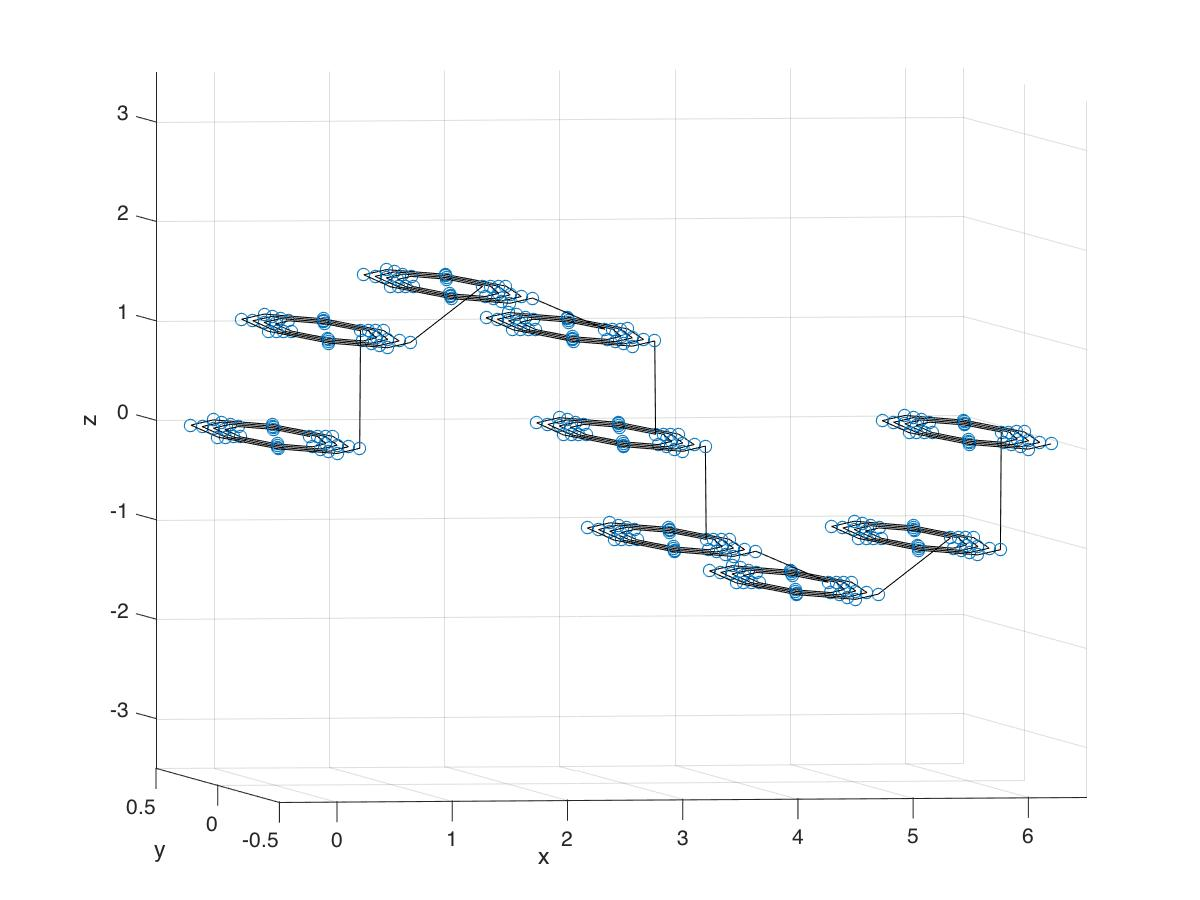
\includegraphics[width=10cm]{NoTilt.jpg}
  \caption{Mesh for \(N_c=8, N_\theta=8, N_t=3\) with no tilt to the slices. Lines connect each coordinate for better visuality.}
\end{figure}

The next step is to rotate the slices appropriately through the angle \(\Theta\) for each slice so that a tubular structure is formed. Only the \(x\) and \(z\) coordinates must be modified. To perform the tilt, the following quantities are computed using trigonometry:

\begin{equation}
\begin{aligned}
w=\sin{(\pi/2-\Theta)}(r+dt)\cos{(\theta)}/\sin{(pi/2)}\\
h = w\sin{(\Theta)}\\
p = w\cos{(\Theta)}\\
\end{aligned}
\end{equation}

To tilt the z-coordinate, for points in the first and fourth quadrant of each slice:

\begin{equation}
z_{new} = z - (-1)^{tube}h
\end{equation}

And for points in the second and third quadrant of each slice:

\begin{equation}
z_{new} = z + (-1)^{tube}h
\end{equation}

where \(tube\) is a variable indicating whether or not the slice is in the left or right half of the tube. For the left half of the tube, \(tube=1\), and in the right half, \(tube=2\).

\item Then, tilt the x-coordinates. For points in the first and fourth quadrants of each slice:

\begin{equation}
x_{new} = x + p
\end{equation}

And for points in the second and third quadrants of each slice:

\begin{equation}
x_{new} = x - p
\end{equation}

\item Finally, tilt the slices that exactly align with the peak and valley of the tube (for odd numbers of \(N_\theta\), this would not be performed). For the slices that align with the peaks and for nodes in the first and fourth quadrants, adjust the \(z\) coordinates according to:

\begin{equation}
z_{new} = z - (r+dt)\cos{(\theta)}
\end{equation}

And for points in the second and third quadrants:

\begin{equation}
z_{new} = z + (r+dt)\cos{(\theta)}
\end{equation}

The \(x\)-coordinates are adjusted by simply setting all of them to the centroid coordinate for that slice. 
\end{enumerate}

This process is fairly complicated, and reveals why meshing software is so valuable. The process here is left fairly general that it can apply for any values of \(N_\theta, N_c, N_t\), but any slight change in the geometry completely invalidates the program. The final mesh for \(N_c=8, N_\theta=8, N_t=3\) is shown below. This mesh is shown because the requested mesh with only \(N_c=4\) is relatively difficult to perceive in a 3-D plot in Matlab, so the following plot better reveals the mesh. Lines are drawn between each coordinate.

\begin{figure}[H]
  \centering
  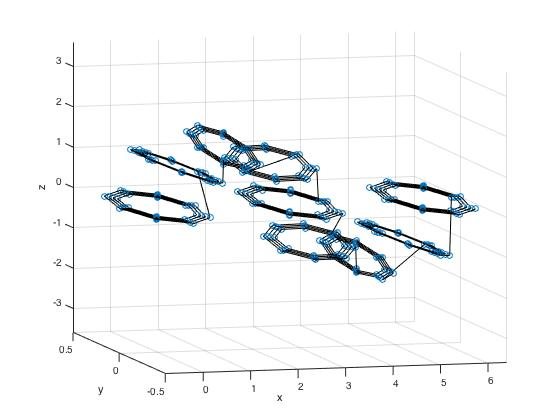
\includegraphics[width=10cm]{RefinedMesh.jpg}
  \caption{Mesh for \(N_c=8, N_\theta=8, N_t=3\). Lines connect each coordinate for better visuality.}
\end{figure}

The coarser mesh, for \(N_c=4, N_\theta=8, N_t=3\) is shown below, again with lines connecting each coordinate for better visibility.

\begin{figure}[H]
  \centering
  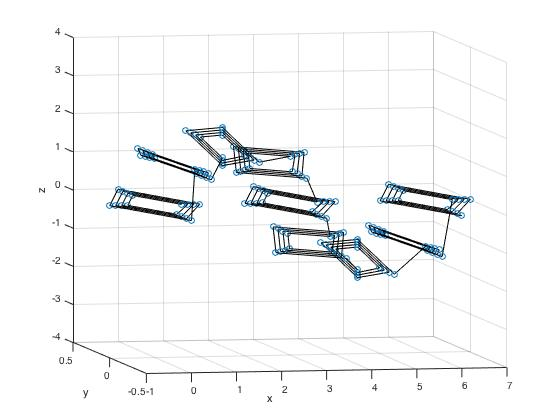
\includegraphics[width=10cm]{CoarseMesh.jpg}
  \caption{Mesh for \(N_c=4, N_\theta=8, N_t=3\). Lines connect each coordinate for better visuality.}
\label{fig:CoarseMesh}
\end{figure}

The mesh in Fig. \ref{fig:CoarseMesh} is shown below without the lines connecting each coordinate.

\begin{figure}[H]
  \centering
  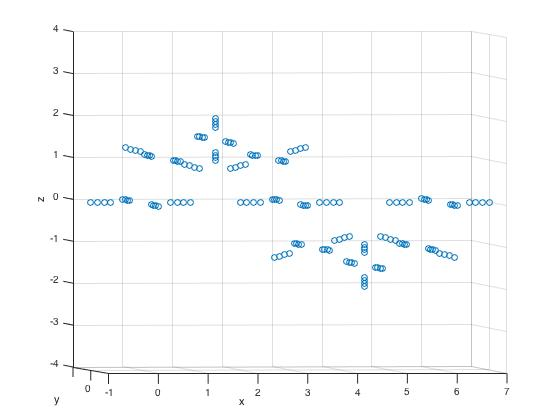
\includegraphics[width=10cm]{CoarseMeshNoLines.jpg}
  \caption{Mesh for \(N_c=4, N_\theta=8, N_t=3\).}
\end{figure}

Note that this assignment did not provide the dimensions of the tube, so I assumed that the inner radius of each arch was 1, the radius of the inner hole of the tube 0.3, and the thickness of the tube 0.2.

\subsection{The Connectivity Matrix}

In order for this mesh to be useful for finite element implementation, a connectivity function must be defined to relate the local node numbering to the global node numbering. The mesh generated numbers the global nodes according to the order in which they were generated. For instance, the first 8 nodes are in the inner layer of the first slice, the next 8 are in the second layer of the first slice, and so on for the first slice. Then, moving to the next \(\Theta\) slice, the node numbering again begins on the inside of the tube and moves counterclockwise in layers until reaching the outside of the tube. This is shown schematically in the figures above by the black lines connecting the coordinates \textit{in the order in which the coordinates are generated}.

The connectivity matrix is an \(N\times8\) matrix, where \(N\) is the total number of elements and 8 is the number of local nodes per element (linear elements are assumed). The local node numbering is performed according to a clockwise fashion. The following schematic shows the node numbering, where the left portion shows the front face, and the right portion shows the back face, all while looking at the front face (i.e. the back face is not written with the perspective of looking at the outward-facing portion of the back face).

\begin{equation}
\begin{aligned}
4 -- 3 & \quad\quad & 8 -- 7\\
2 -- 1 & \quad\quad & 6 -- 5\\
\end{aligned}
\end{equation}

So, for each slice, the nodes on the face of each element can be determined using a numbering scheme that follows the order in which the nodes were defined. Beginning with \(\theta=0\), and moving counterclockwise, the local nodes are numbered, moving progressively outwards in the layers until reaching the last node for a particular slice. 

There are \(N_t\cdot N_c\cdot N_\theta\) total elements. For each slice, the nodes are numbered moving counterclockwise, beginning at the same node that is meshed first. After each layer is complete, the numbering moves to the next layer in the same fashion. Once an entire slice is complete, the next slice is also meshed. This defines only the \textit{frontal} node numberings shown in the above equation. For example, for \(N_\theta=2, N_t=3, N_c=4\), the connectivity matrix \(\textbf{LM}\) looks like the following \textit{before} the nodes on the backs of the first 12 elements are related to the nodes on the fronts of the next 12 elements.

\begin{equation}
\textbf{LM}=
\begin{bmatrix}
1 & 2 & 5 & 6 & 0 & 0 & 0 & 0\\
2 & 3 & 6 & 7 & 0 & 0 & 0 & 0\\
3 & 4 & 7 & 8 & 0 & 0 & 0 & 0\\
4 & 1 & 8 & 5 & 0 & 0 & 0 & 0\\
5 & 6 & 9 & 10 & 0 & 0 & 0 & 0\\
6 & 7 & 10 & 11 & 0 & 0 & 0 & 0\\
7 & 8 & 11 & 12 & 0 & 0 & 0 & 0\\
8 & 5 & 12 & 9 & 0 & 0 & 0 & 0\\
9 & 10 & 13 & 14 & 0 & 0 & 0 & 0\\
10 & 11 & 14 & 15 & 0 & 0 & 0 & 0\\
11 & 12 & 15 & 16 & 0 & 0 & 0 & 0\\
12 & 9 & 16 & 13 & 0 & 0 & 0 & 0\\
17 & 18 & 21 & 22 & 0 & 0 & 0 & 0\\
18 & 19 & 22 & 23 & 0 & 0 & 0 & 0\\
19 & 20 & 23 & 24 & 0 & 0 & 0 & 0\\
20 & 17 & 24 & 21 & 0 & 0 & 0 & 0\\
21 & 22 & 25 & 26 & 0 & 0 & 0 & 0\\
22 & 23 & 26 & 27 & 0 & 0 & 0 & 0\\
23 & 24 & 27 & 28 & 0 & 0 & 0 & 0\\
24 & 21 & 28 & 25 & 0 & 0 & 0 & 0\\
25 & 26 & 29 & 30 & 0 & 0 & 0 & 0\\
26 & 27 & 30 & 31 & 0 & 0 & 0 & 0\\
27 & 28 & 31 & 32 & 0 & 0 & 0 & 0\\
28 & 25 & 32 & 29 & 0 & 0 & 0 & 0\\
33 & 34 & 37 & 38 & 0 & 0 & 0 & 0\\
34 & 35 & 38 & 39 & 0 & 0 & 0 & 0\\
35 & 36 & 39 & 40 & 0 & 0 & 0 & 0\\
36 & 33 & 40 & 37 & 0 & 0 & 0 & 0\\
37 & 38 & 41 & 42 & 0 & 0 & 0 & 0\\
38 & 39 & 42 & 43 & 0 & 0 & 0 & 0\\
39 & 40 & 43 & 44 & 0 & 0 & 0 & 0\\
40 & 37 & 44 & 41 & 0 & 0 & 0 & 0\\
41 & 42 & 45 & 46 & 0 & 0 & 0 & 0\\
42 & 43 & 46 & 47 & 0 & 0 & 0 & 0\\
43 & 44 & 47 & 48 & 0 & 0 & 0 & 0\\
44 & 41 & 48 & 45 & 0 & 0 & 0 & 0\\
\end{bmatrix}
\end{equation}

This is not the final form for the connectivity matrix (a.k.a. location matrix). Because the slices lay exactly on top of one another, the front nodes of the second slice are exactly the back nodes on the previous slice. With this knowledge, the back nodes for each element can be assigned based on the frontal nodes of the following slice. Then, the last \(N_cN_t\) rows in the location matrix above can be deleted, since they refer to the frontal nodes of a slice that does not technically exist (there are only 2 slices, but 3 planes defining those slices). With this information, the final form of the location matrix becomes, for \(N_\theta=2, N_t=3, N_c=4\) for example:

\begin{equation}
\textbf{LM}=
\begin{bmatrix}
1 & 2 & 5 & 6 & 17 & 18 & 21 & 22\\
2 & 3 & 6 & 7 & 18 & 19 & 22 & 23\\
3 & 4 & 7 & 8 & 19 & 20 & 23 & 24\\
4 & 1 & 8 & 5 & 20 & 17 & 24 & 21\\
5 & 6 & 9 & 10 & 21 & 22 & 25 & 26\\
6 & 7 & 10 & 11 & 22 & 23 & 26 & 27\\
7 & 8 & 11 & 12 & 23 & 24 & 27 & 28\\
8 & 5 & 12 & 9 & 24 & 21 & 28 & 25\\
9 & 10 & 13 & 14 & 25 & 26 & 29 & 30\\
10 & 11 & 14 & 15 & 26 & 27 & 30 & 31\\
11 & 12 & 15 & 16 & 27 & 28 & 31 & 32\\
12 & 9 & 16 & 13 & 28 & 25 & 32 & 29\\
17 & 18 & 21 & 22 & 33 & 34 & 37 & 38\\
18 & 19 & 22 & 23 & 34 & 35 & 38 & 39\\
19 & 20 & 23 & 24 & 35 & 36 & 39 & 40\\
20 & 17 & 24 & 21 & 36 & 33 & 40 & 37\\
21 & 22 & 25 & 26 & 37 & 38 & 41 & 42\\
22 & 23 & 26 & 27 & 38 & 39 & 42 & 43\\
23 & 24 & 27 & 28 & 39 & 40 & 43 & 44\\
24 & 21 & 28 & 25 & 40 & 37 & 44 & 41\\
25 & 26 & 29 & 30 & 41 & 42 & 45 & 46\\
26 & 27 & 30 & 31 & 42 & 43 & 46 & 47\\
27 & 28 & 31 & 32 & 43 & 44 & 47 & 48\\
28 & 25 & 32 & 29 & 44 & 41 & 48 & 45\\
\end{bmatrix}
\end{equation}

Each row in the location matrix corresponds to an elements, and each column to a local node number, so that \(LM(1,4)\) indicates the global node number of local node number 4 in element 1. This method is extended to the case for \(N_\theta=8, N_c=4, N_t=3\), where the purpose of the previous discussion for a fewer number of circumferential elements was simply to illustrate the process by which the location matrix is generated. So, for the problem statement in this homework assignment (\(N_\theta=8, N_c=4, N_t=3\)):

\begin{equation}
\label{eq:LMFinalForm}
\textbf{LM}=
\begin{bmatrix}LM_1 \\ LM_2\end{bmatrix}
\end{equation}

where, in order to be able to print the matrix, the following components are defined to simply be stacked on top of each other as in Eq. \eqref{eq:LMFinalForm}.

\begin{equation}
LM_1=
\begin{bmatrix}
1 & 2 & 5 & 6 & 17 & 18 & 21 & 22\\
2 & 3 & 6 & 7 & 18 & 19 & 22 & 23\\
3 & 4 & 7 & 8 & 19 & 20 & 23 & 24\\
4 & 1 & 8 & 5 & 20 & 17 & 24 & 21\\
5 & 6 & 9 & 10 & 21 & 22 & 25 & 26\\
6 & 7 & 10 & 11 & 22 & 23 & 26 & 27\\
7 & 8 & 11 & 12 & 23 & 24 & 27 & 28\\
8 & 5 & 12 & 9 & 24 & 21 & 28 & 25\\
9 & 10 & 13 & 14 & 25 & 26 & 29 & 30\\
10 & 11 & 14 & 15 & 26 & 27 & 30 & 31\\
11 & 12 & 15 & 16 & 27 & 28 & 31 & 32\\
12 & 9 & 16 & 13 & 28 & 25 & 32 & 29\\
17 & 18 & 21 & 22 & 33 & 34 & 37 & 38\\
18 & 19 & 22 & 23 & 34 & 35 & 38 & 39\\
19 & 20 & 23 & 24 & 35 & 36 & 39 & 40\\
20 & 17 & 24 & 21 & 36 & 33 & 40 & 37\\
21 & 22 & 25 & 26 & 37 & 38 & 41 & 42\\
22 & 23 & 26 & 27 & 38 & 39 & 42 & 43\\
23 & 24 & 27 & 28 & 39 & 40 & 43 & 44\\
24 & 21 & 28 & 25 & 40 & 37 & 44 & 41\\
25 & 26 & 29 & 30 & 41 & 42 & 45 & 46\\
26 & 27 & 30 & 31 & 42 & 43 & 46 & 47\\
27 & 28 & 31 & 32 & 43 & 44 & 47 & 48\\
28 & 25 & 32 & 29 & 44 & 41 & 48 & 45\\
33 & 34 & 37 & 38 & 49 & 50 & 53 & 54\\
34 & 35 & 38 & 39 & 50 & 51 & 54 & 55\\
35 & 36 & 39 & 40 & 51 & 52 & 55 & 56\\
36 & 33 & 40 & 37 & 52 & 49 & 56 & 53\\
37 & 38 & 41 & 42 & 53 & 54 & 57 & 58\\
38 & 39 & 42 & 43 & 54 & 55 & 58 & 59\\
39 & 40 & 43 & 44 & 55 & 56 & 59 & 60\\
40 & 37 & 44 & 41 & 56 & 53 & 60 & 57\\
41 & 42 & 45 & 46 & 57 & 58 & 61 & 62\\
42 & 43 & 46 & 47 & 58 & 59 & 62 & 63\\
43 & 44 & 47 & 48 & 59 & 60 & 63 & 64\\
44 & 41 & 48 & 45 & 60 & 57 & 64 & 61\\
49 & 50 & 53 & 54 & 65 & 66 & 69 & 70\\
50 & 51 & 54 & 55 & 66 & 67 & 70 & 71\\
51 & 52 & 55 & 56 & 67 & 68 & 71 & 72\\
52 & 49 & 56 & 53 & 68 & 65 & 72 & 69\\
53 & 54 & 57 & 58 & 69 & 70 & 73 & 74\\
54 & 55 & 58 & 59 & 70 & 71 & 74 & 75\\
55 & 56 & 59 & 60 & 71 & 72 & 75 & 76\\
56 & 53 & 60 & 57 & 72 & 69 & 76 & 73\\
57 & 58 & 61 & 62 & 73 & 74 & 77 & 78\\
58 & 59 & 62 & 63 & 74 & 75 & 78 & 79\\
59 & 60 & 63 & 64 & 75 & 76 & 79 & 80\\
60 & 57 & 64 & 61 & 76 & 73 & 80 & 77\\
65 & 66 & 69 & 70 & 81 & 82 & 85 & 86\\
\end{bmatrix}
\end{equation}

\begin{equation}
LM_2=
\begin{bmatrix}
66 & 67 & 70 & 71 & 82 & 83 & 86 & 87\\
67 & 68 & 71 & 72 & 83 & 84 & 87 & 88\\
68 & 65 & 72 & 69 & 84 & 81 & 88 & 85\\
69 & 70 & 73 & 74 & 85 & 86 & 89 & 90\\
70 & 71 & 74 & 75 & 86 & 87 & 90 & 91\\
71 & 72 & 75 & 76 & 87 & 88 & 91 & 92\\
72 & 69 & 76 & 73 & 88 & 85 & 92 & 89\\
73 & 74 & 77 & 78 & 89 & 90 & 93 & 94\\
74 & 75 & 78 & 79 & 90 & 91 & 94 & 95\\
75 & 76 & 79 & 80 & 91 & 92 & 95 & 96\\
76 & 73 & 80 & 77 & 92 & 89 & 96 & 93\\
81 & 82 & 85 & 86 & 97 & 98 & 101 & 102\\
82 & 83 & 86 & 87 & 98 & 99 & 102 & 103\\
83 & 84 & 87 & 88 & 99 & 100 & 103 & 104\\
84 & 81 & 88 & 85 & 100 & 97 & 104 & 101\\
85 & 86 & 89 & 90 & 101 & 102 & 105 & 106\\
86 & 87 & 90 & 91 & 102 & 103 & 106 & 107\\
87 & 88 & 91 & 92 & 103 & 104 & 107 & 108\\
88 & 85 & 92 & 89 & 104 & 101 & 108 & 105\\
89 & 90 & 93 & 94 & 105 & 106 & 109 & 110\\
90 & 91 & 94 & 95 & 106 & 107 & 110 & 111\\
91 & 92 & 95 & 96 & 107 & 108 & 111 & 112\\
92 & 89 & 96 & 93 & 108 & 105 & 112 & 109\\
97 & 98 & 101 & 102 & 113 & 114 & 117 & 118\\
98 & 99 & 102 & 103 & 114 & 115 & 118 & 119\\
99 & 100 & 103 & 104 & 115 & 116 & 119 & 120\\
100 & 97 & 104 & 101 & 116 & 113 & 120 & 117\\
101 & 102 & 105 & 106 & 117 & 118 & 121 & 122\\
102 & 103 & 106 & 107 & 118 & 119 & 122 & 123\\
103 & 104 & 107 & 108 & 119 & 120 & 123 & 124\\
104 & 101 & 108 & 105 & 120 & 117 & 124 & 121\\
105 & 106 & 109 & 110 & 121 & 122 & 125 & 126\\
106 & 107 & 110 & 111 & 122 & 123 & 126 & 127\\
107 & 108 & 111 & 112 & 123 & 124 & 127 & 128\\
108 & 105 & 112 & 109 & 124 & 121 & 128 & 125\\
113 & 114 & 117 & 118 & 129 & 130 & 133 & 134\\
114 & 115 & 118 & 119 & 130 & 131 & 134 & 135\\
115 & 116 & 119 & 120 & 131 & 132 & 135 & 136\\
116 & 113 & 120 & 117 & 132 & 129 & 136 & 133\\
117 & 118 & 121 & 122 & 133 & 134 & 137 & 138\\
118 & 119 & 122 & 123 & 134 & 135 & 138 & 139\\
119 & 120 & 123 & 124 & 135 & 136 & 139 & 140\\
120 & 117 & 124 & 121 & 136 & 133 & 140 & 137\\
121 & 122 & 125 & 126 & 137 & 138 & 141 & 142\\
122 & 123 & 126 & 127 & 138 & 139 & 142 & 143\\
123 & 124 & 127 & 128 & 139 & 140 & 143 & 144\\
124 & 121 & 128 & 125 & 140 & 137 & 144 & 141\\
\end{bmatrix}
\end{equation}

\section{Appendix}

This section contains the complete code used in this assignment. 

\subsection{\texttt{MeshGenerator.m}}
This program generates the mesh and connectivity matrix.
\lstinputlisting[language=Matlab]{MeshGenerator.m}

\end{document}